\chapter{Знакомство с Lego Digital Designer}
{\bfseries Анонс:}\\\\
Названия деталей. Lego Digital Designer: установка и первые модели.
{\bfseries Цели:}
\begin{itemize}
	\item{}{\bfseries Обучающие:} Закрепить  знание основных терминов. Обучить основам работы в Lego Digital Designer. 
	\item{}{\bfseries \yellowText{\greenText{Развивающие:}}} \\
\end{itemize}	
{\bfseries Ход занятия:}\\\\
\begin{tabular}{lll}
	\hyperlink{lesson3x1}{1. Организационный момент} & Презентация & (5 мин)\\
	\hyperlink{lesson3x2}{2. Названия деталей} & Игра & (15 мин) \\
	\hyperlink{lesson3x3}{3. Lego Digital Designer} & Презентация & (45 мин) \\
	\hyperlink{lesson3x4}{4. Модель совы} & Практика & (50 мин)\\
\end{tabular}\\\\

{\hypertarget{lesson3x1}{\blackBlueText{I.Организационный момент}}}\\\\

Сегодня для работы каждому ребенку понадобятся компьютеры, с установленным на них Lego Digital Designer. Оптимальным является вариант компьютеров, объединенных во внутреннюю сеть, с возможностью создания каждому ребенку личного аrкаунта, блокировки доступа в интернет и к части жесткого диска.\\\\

{\hypertarget{lesson3x2}{\blackBlueText{II. Названия деталей}}}\\\\

Для закрепления материала предыдущего занятия и настройки на рабочий лад предлагается провести следующую игру. В шляпу складываются разные детали набора, из расчета 5--6 штук на одного игрока. У каждого игрока есть 30 секунд, что бы вынимая по очереди из шляпы детали называть их. Назвал правильно~--- получаешь очко, нет~--- кидаешь обратно в шляпу. По истечении 30 секунд шляпа переходит следующему. Игра продолжается пока не закончатся все детали.\\\\

{\hypertarget{lesson3x3}{\blackBlueText{III. Lego Digital Designer}}}\\\\

{\bfseries LEGO Digital Designer (LDD)}~--- это программа, представляющая собой виртуальный конструктор LEGO, с помощью которого можно собирать всевозможные 3D-модели. Как и в реальном конструкторе в {\bfseries LDD} присутствует богатый выбор разнообразных деталей, которые можно скреплять друг с другом. Рабочую область программы можно приближать, удалять и разворачивать под любым углом.

Программа распространяется бесплатно, установочный файл можно скачать с
\href{http://ldd.lego.com/nb-no/download/}{\whiteBlueText{\underline{http://ldd.lego.com/nb-no/download/}}}.
\begin{figure}[h!]
	\begin{center}
		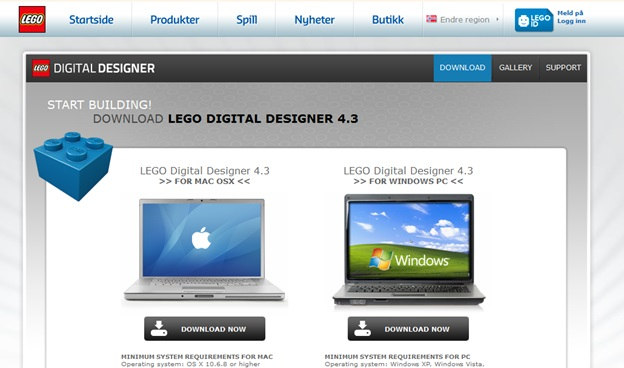
\includegraphics[width=1\linewidth]{chapters/chapter3/images/1}
		\caption{}
		\label{ris:image3x1}
	\end{center}
\end{figure}

Так же версию LDD 4.3 для Windows PC можно найти в папке LDD мультимедийных материалов к настоящему пособию.
\clearpage
Создание моделей  роботов в LDD полезно по следующим причинам:
\begin{itemize}
	\item Прививается навык анализа конструкции. Реальные детали можно соединить абы как, « по вдохновению», но создавая модель придется осознать, как это было сделано.
	\item Прививается навык продумывания конструкции. Создавая дома модель робота к следующему занятию есть возможность перебрать множество вариантов.
	\item Развивается пространственное мышление.
	\item Прививается навык работы в инженерных средах. В настоящем конструировании и роботостроении не обойтись без серьезных расчетов в различных программных пакетах и создания моделей частей устройства. Использование LDD подготавливает детей к работе в подобных программах.
	\item Наличие  сохраненной модели индивидуального проекта позволяет другому ребенку ознакомиться с техническими решениями, использованными в конструкции и, при необходимости, воспроизвести отдельные узлы или всего робота.
\end{itemize}

{\slshape В рамках настоящего курса предлагается следующий алгоритм взаимодействия с LDD. На втором занятии дети  в классе, фронтально обучаются работе в LDD по предложенной ниже инструкции. Затем они учатся разбираться с чужой моделью (Занятие 3) и создавать свои (Занятиям 7 и 8). Далее при работе над соревновательными и творческими задачами модель конструкции в LDD становится обязательной частью технической документации проекта.}\\
Для того чтобы начать работу в LDD, запустим его и выберем вкладку Lego Mindstorms.
\begin{figure}[h!]
	\begin{center}
		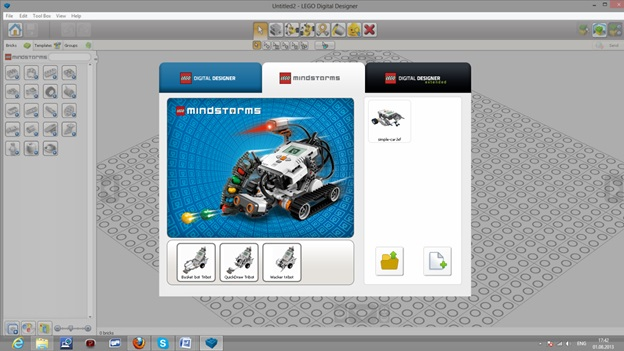
\includegraphics[width=0.76\linewidth]{chapters/chapter3/images/2}
		\caption{}
		\label{ris:image3x2}
	\end{center}
\end{figure}	

Кликнем по значку чистого листа (free build) в правом нижнем углу и создадим новый проект.
\begin{figure}[h!]
	\begin{center}
		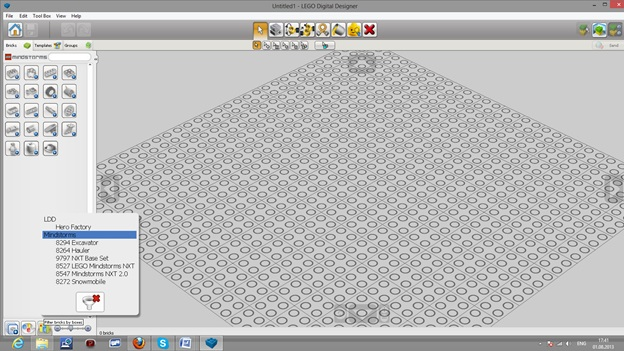
\includegraphics[width=0.8\linewidth]{chapters/chapter3/images/3}
		\caption{}
		\label{ris:image3x3}
	\end{center}
\end{figure}

В левом нижнем углу, под списком деталей, выберем Filter bricks by box (желтый значок) и выберем имеющийся у нас набор.
\begin{figure}[h!]
	\begin{center}
		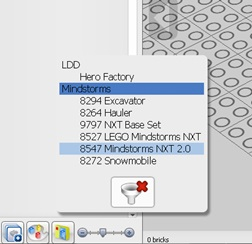
\includegraphics[width=0.65\linewidth]{chapters/chapter3/images/4}
		\caption{}
		\label{ris:image3x4}
	\end{center}
\end{figure}	

Количество доступных деталей уменьшиться, теперь их ровно столько же, сколько в нашем наборе.\\

{\hypertarget{lesson3x3}{\blackBlueText{IV. Модель совы}}}\\\\

{\bfseries Работа идет в режиме «наблюдай за мной, повторяй за мной». Преподаватель по шагам показывает, что нужно делать, выводя экран своего компьютера на проектор. После каждого шага учащимся предоставляется несколько минут, чтобы повторить действия преподавателя.}

\begin{enumerate}
	\item Сохраним файл. Для этого выбираем вкладку File->Save as \dots
	\begin{figure}[h!]
		\begin{center}
			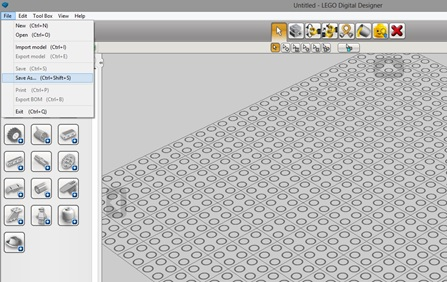
\includegraphics[width=1\linewidth]{chapters/chapter3/images/5}
			\caption{}
			\label{ris:image3x5}
		\end{center}
	\end{figure}
	\clearpage
	Выбираем папку, в которую хотим сохранить проект, и пишем его имя.
	\begin{figure}[h!]
		\begin{center}
			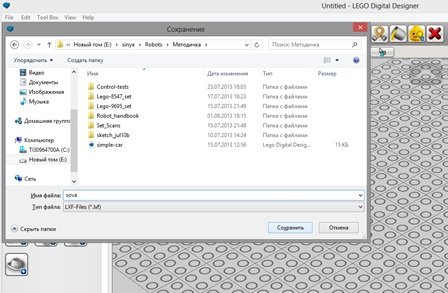
\includegraphics[width=1\linewidth]{chapters/chapter3/images/6}
			\caption{}
			\label{ris:image3x6}
		\end{center}
	\end{figure}
	Видим, что в заголовке имя тоже поменялось.
	\begin{figure}[h!]
		\begin{center}
			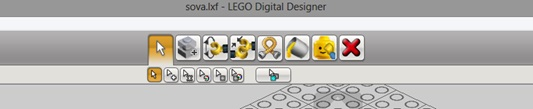
\includegraphics[width=1\linewidth]{chapters/chapter3/images/7}
			\caption{}
			\label{ris:image3x7}
		\end{center}
	\end{figure}
	\clearpage
	\item Выбираем балку с 5 отверстиями.
	\begin{figure}[h!]
		\begin{center}
			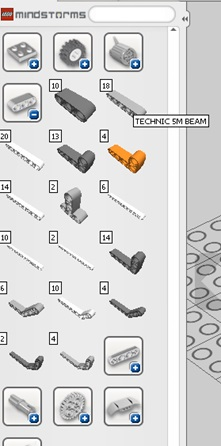
\includegraphics[width=0.7\linewidth]{chapters/chapter3/images/8}
			\caption{}
			\label{ris:image3x8}
		\end{center}
	\end{figure}
	Кладем ее на поле для сборки. По умолчанию она ложится горизонтально. С помощью стрелочек на клавиатуре поворачиваем ее на 90 градусов.
	\begin{figure}[h!]
		\begin{center}
			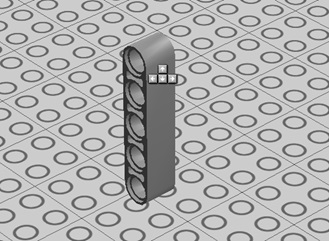
\includegraphics[width=0.79\linewidth]{chapters/chapter3/images/9}
			\caption{}
			\label{ris:image3x9}
		\end{center}
	\end{figure}
	\item Выбираем синий штифт и вставляем его в нижнее отверстие балки. Когда детали стыкуются, они подсвечиваются зеленой рамкой.
	\begin{figure}[h!]
		\begin{center}
			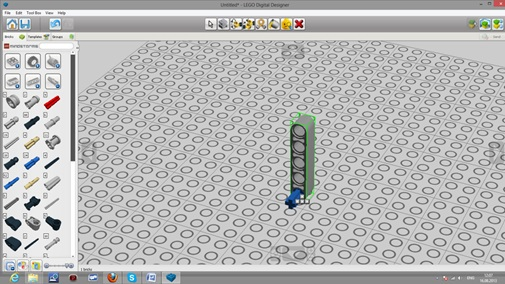
\includegraphics[width=1\linewidth]{chapters/chapter3/images/10}
			\caption{}
			\label{ris:image3x10}
		\end{center}
	\end{figure}
	\item Выбираем самую большую серую шестеренку и одеваем ее на штифт. В стандартном наборе нет серых шестеренок, есть аналогичная черная. Из эстетических соображений  в рассматриваемом примере сняты фильтры «by box» и собирается серая сова.
	\begin{figure}[h!]
		\begin{center}
			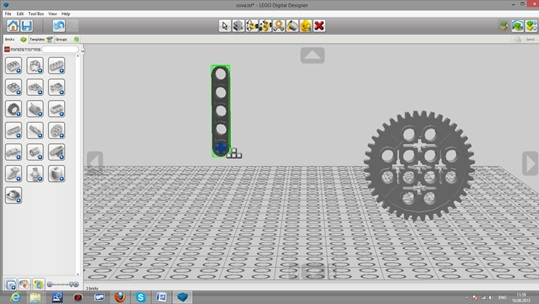
\includegraphics[width=1\linewidth]{chapters/chapter3/images/11}
			\caption{}
			\label{ris:image3x11}
		\end{center}
	\end{figure}
	\begin{figure}[h!]
		\begin{center}
			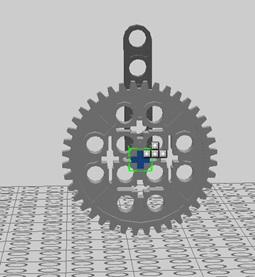
\includegraphics[width=0.55\linewidth]{chapters/chapter3/images/12}
			\caption{}
			\label{ris:image3x12}
		\end{center}
	\end{figure}
	\item Одеваем красный штифт и маленькую шестеренку.\\\\
	\begin{figure}[h!]
		\begin{center}
			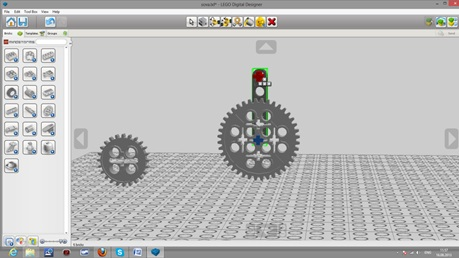
\includegraphics[width=1\linewidth]{chapters/chapter3/images/13}
			\caption{}
			\label{ris:image3x13}
		\end{center}
	\end{figure}
	\begin{figure}[h!]
		\begin{center}
			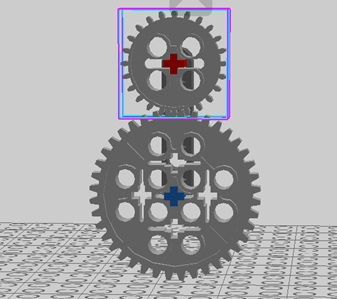
\includegraphics[width=0.67\linewidth]{chapters/chapter3/images/14}
			\caption{}
			\label{ris:image3x14}
		\end{center}
	\end{figure}
	При необходимости выбираем на верхней панели инструмент Hinge tool (H) и вращаем шестеренку, до зацепления зубцами.
	\item Укрепляем конструкцию еще одним синим штифтом. Добавляем ось со втулкой.
	\begin{figure}[h!]
		\begin{center}
			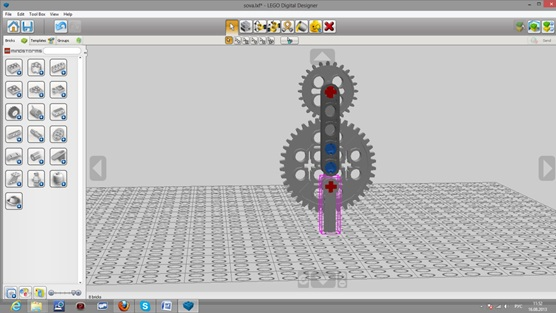
\includegraphics[width=1\linewidth]{chapters/chapter3/images/15}
			\caption{}
			\label{ris:image3x15}
		\end{center}
	\end{figure}
	\item Надеваем на ось балку с тремя отверстиями.
	\begin{figure}[h!]
		\begin{center}
			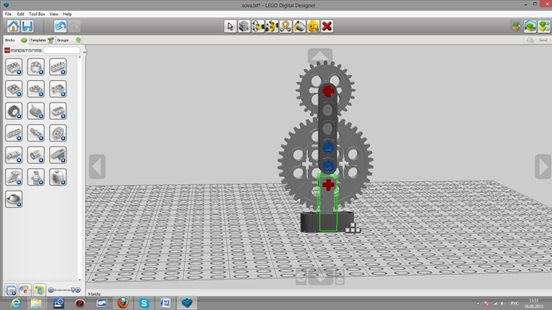
\includegraphics[width=1\linewidth]{chapters/chapter3/images/16}
			\caption{}
			\label{ris:image3x16}
		\end{center}
	\end{figure}
	\clearpage
	\item Добавляем черные штифты.
	\begin{figure}[h!]
		\begin{center}
			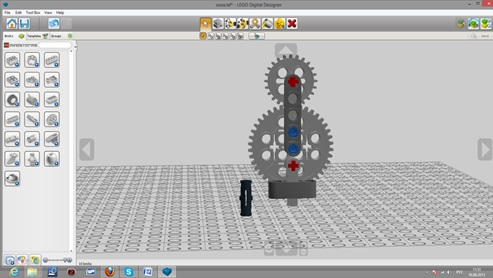
\includegraphics[width=1\linewidth]{chapters/chapter3/images/17}
			\caption{}
			\label{ris:image3x17}
		\end{center}
	\end{figure}
	\item Сажаем на пару черных штифтов крылья.
	\begin{figure}[h!]
		\begin{center}
			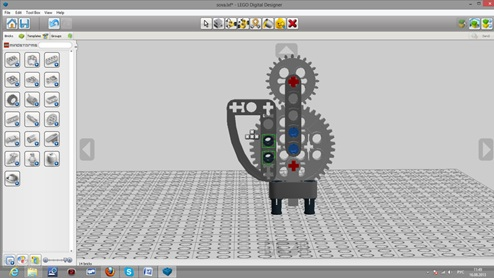
\includegraphics[width=1\linewidth]{chapters/chapter3/images/18}
			\caption{}
			\label{ris:image3x18}
		\end{center}
	\end{figure}
	\clearpage
	\item Добавляем соединители~--- лапы.
	\begin{figure}[h!]
		\begin{center}
			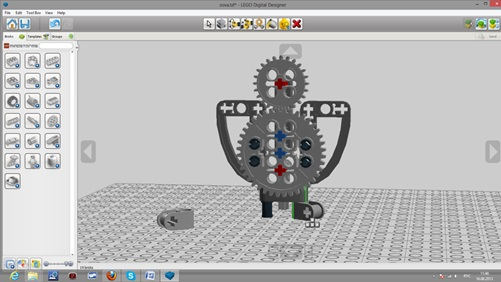
\includegraphics[width=1\linewidth]{chapters/chapter3/images/19}
			\caption{}
			\label{ris:image3x19}
		\end{center}
	\end{figure}
	\item Вставляем бежевые глаза.
	\begin{figure}[h!]
		\begin{center}
			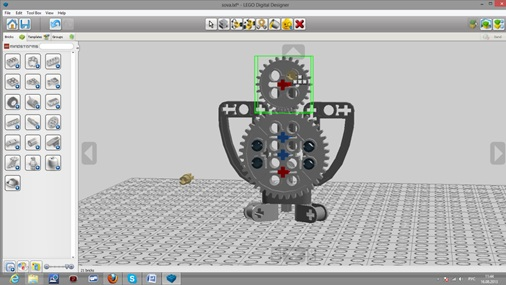
\includegraphics[width=1\linewidth]{chapters/chapter3/images/20}
			\caption{}
			\label{ris:image3x20}
		\end{center}
	\end{figure}
	\clearpage
	\item Сова готова!
	\begin{figure}[h!]
		\begin{center}
			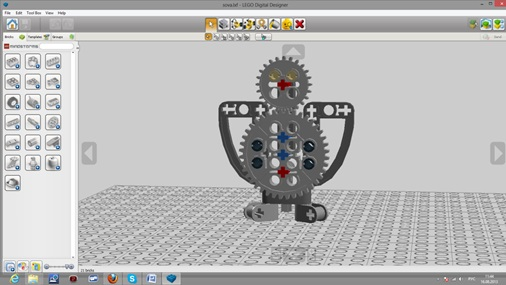
\includegraphics[width=1\linewidth]{chapters/chapter3/images/21}
			\caption{}
			\label{ris:image3x21}
		\end{center}
	\end{figure}
\end{enumerate}

{\slshape Можно дать детям немного свободного времени на усовершенствование совы~--- сделать ей клюв, уши, гнездо.}

В LDD есть очень полезная опция~--- Building guide mode, выбираемый в правом верхнем углу.
\begin{figure}[h!]
	\begin{center}
		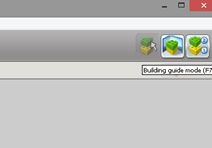
\includegraphics[width=0.75\linewidth]{chapters/chapter3/images/22}
		\caption{}
		\label{ris:image3x22}
	\end{center}
\end{figure}

В этом режиме программа по шагам можно проиграть, созданную программой инструкцию по сборке модели. Это бывает очень полезно при ознакомлении с чужой моделью и необходимости ее воспроизводства.
\begin{figure}[h!]
	\begin{center}
		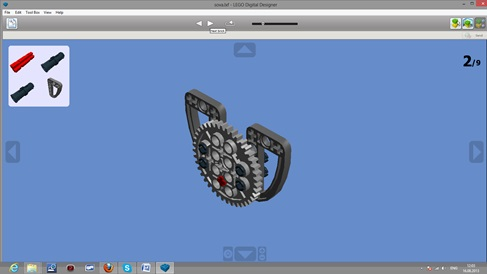
\includegraphics[width=1\linewidth]{chapters/chapter3/images/23}
		\caption{}
		\label{ris:image3x23}
	\end{center}
\end{figure}

Теперь предложите детям взять наборы и собрать сову в реальности, исполняя те шаги, которые предложит компьютер.